\chapter{Mathematical models of Bose-Einstein condensates}

In this chapter we provide the theoretical background necessary to understand
the dynamics of ultracold atomic gases.
We start by introducing the most simple form of a Bose-Einstein condensate,
the scalar condensate.
This lays the framework for building to more complex systems.
We then go on to discuss the two-component condensate, where additional
interactions arise between atoms of differing components.
Finally, we construct the framework needed to understand spinor BECs, which is
the main basis of this thesis.

\section{Scalar Bose-Einstein condensates}
\subsection{Mean-field description}
A system of \(N\) particles interacting through binary collisions is described
by an \(N\)-body Schr\"{o}dinger equation, given as
\begin{equation}
    i\hbar \pdv{}{t}\Psi(\vb{r}_1;\ldots;\vb{r}_N, t) =
    \hat{H}_N\Psi(\vb{r}_1;\ldots;\vb{r}_N, t),
\end{equation}
where the \(N\)-body Hamiltonian operator is given by
\begin{equation}
    \hat{H}_N = -\sum_i \frac{\hbar^2}{2m}\nabla_i^2
    + \sum_{i \neq j}V(\vb{r}_i - \vb{r}_j).
\end{equation}
The first sum of the above equation represents the kinetic energy operator,
whilst the second describes the two-body potential operator.
This description, however, becomes unwieldy when trying to model the number of
particles associated with typical BEC experiments.

Instead, we model the system using a mean-field theory, in which we make two
assumptions.
Firstly, the dilute nature of a BEC justifies that any binary interaction
between two particles at positions \(\vb{r}_1, \vb{r}_2\) takes the form of
a contact interaction modelled by the following delta function:
\begin{equation}
    V(\vb{r}_1 - \vb{r}_2) = g\delta(\vb{r}_1 - \vb{r}_2),
\end{equation}
where \(g\) represents an interaction coefficient.
Secondly, we assume that, for sufficiently low temperatures, the system
undergoes Bose-Einstein condensation, and all particles of
the system occupy the same quantum state.
This implies that each particle is described by the same single-particle wave
function and hence the system can be described by a macroscopic wave function
\(\psi(\vb{r}, t)\) for position \(\vb{r}\) and time \(t\).
Additionally, the field \(\psi \) is scalar since each particle shares the same
phase and quantum state.
This approximation is only valid in the limit of zero temperature, where there
are no particles contributing to thermal or quantum fluctuations beyond the
classical field.

\subsection{The Gross-Pitaevskii equation}
The preceding assumptions form the basis of constructing the underlying equation
that governs the dynamics of Bose-Einstein condensate systems: the
Gross-Pitaevskii equation (GPE):
\begin{equation}\label{eq: scalar-GPE}
    i\hbar \pdv{\psi(\vb{r}, t)}{t} = \left(-\frac{\hbar^2}{2m}\nabla^2
    + V(\vb{r}, t) +g|\psi(\vb{r}, t)|^2\right)\psi(\vb{r}, t),
\end{equation}
where \(V(\vb{r}, t)\) is a trapping potential.

The first two terms on the right-hand side describe the energy of a single
particle in an external potential.
The third term accounts for the interactions within the condensate, where
\(g=4\pi \hbar^2a_s/m\) is the interaction strength of the condensate for
s-wave scattering length \(a_s\) and atomic mass \(m\).
For \(g>0\) the interactions are repulsive and for \(g < 0\) attractive.
When \(g=0\) there are no interactions present and the system reduces to the
Schr\"{o}dinger equation.

The wave function of the system is normalised to the number of particles
\begin{equation}
    \int |\psi(\vb{r}, t)|^2 d\vb{r} = N.
\end{equation}
The total mass of the condensate is given as \(M=mN\), where \(N\) is provided
by the above normalisation condition.

The energy of the system is
\begin{equation}
    E = \int d^3\vb{r} \left[\frac{\hbar^2}{2m}|\nabla\psi|^2
        + V|\psi|^2 + \frac{g}{2}|\psi|^4\right]
    = E_\mathrm{kin} + E_\mathrm{pot} + E_\mathrm{int},
\end{equation}
where \(E_\mathrm{kin}, E_\mathrm{pot}\) and \(E_\mathrm{int}\) describes the
kinetic, potential, and interaction energies, respectively.

\section{Two-component Bose-Einstein condensates}
We now generalise part of the theory introduced in the previous section to
describe multi-component condensates.
The time-dependent coupled Gross-Pitaevskii equations each describe a condensate
similar to the standard GPE, but now with an additional non-linear term that
describes the interactions of atoms between condensate components.
The coupled GPEs are given as
\begin{equation}\label{eq: two-component-GPEs}
    \begin{aligned}
        i\hbar \pdv{\psi_1(\vb{r}, t)}{t} & =
        \left[-\frac{\hbar^2}{2m_1}\nabla^2 + V_1(\vb{r}, t)
            + g_1|\psi_1(\vb{r}, t)|^2
        + g_{12}|\psi_2(\vb{r}, t)|^2\right]\psi_1(\vb{r}, t) \\
        i\hbar \pdv{\psi_2(\vb{r}, t)}{t} & =
        \left[-\frac{\hbar^2}{2m_2}\nabla^2 + V_2(\vb{r}, t)
            + g_2|\psi_2(\vb{r}, t)|^2
            + g_{12}|\psi_1(\vb{r}, t)|^2\right]\psi_2(\vb{r}, t),
    \end{aligned}
\end{equation}
where \(\psi_j(\vb{r}, t)\) describes component \(j\) with atomic mass \(m_j\)
for \(j=1, 2\) and \(V(\vb{r}, t)\) is an external trapping potential.
Additionally, the interaction terms are given as
\begin{equation}
    g_j = \frac{4\pi \hbar^2a_j}{2m_j}, \qquad
    g_{12} = g_{21} = \frac{2\pi\hbar^2(m_1+m_2)a_{12}}{m_1m_2},
\end{equation}
which describe the intra-species and inter-species interaction strengths,
respectively.
Similar to the scalar case, the wave function of each component is normalised
to the number of atoms of that component
\begin{equation}
    \int |\psi_j|^2 d^3\vb{r} = N_j.
\end{equation}

The time-independent GPEs are obtained through the substitution
\(\psi_j(\vb{r}, t)=\psi_j(\vb{r})e^{-i\mu_j t/\hbar}\) in
Eq.~\eqref{eq: two-component-GPEs}, yielding
\begin{equation}\label{eq: time-indep-two-component-GPEs}
    \begin{aligned}
        \mu_1\psi_1(\vb{r}) & =
        \left[-\frac{\hbar^2}{2m_1}\nabla^2 + V_1(\vb{r})
            + g_1|\psi_1(\vb{r})|^2
        + g_{12}|\psi_2(\vb{r})|^2\right]\psi_1(\vb{r}) \\
        \mu_2\psi_2(\vb{r}) & =
        \left[-\frac{\hbar^2}{2m_2}\nabla^2 + V_2(\vb{r})
            + g_2|\psi_2(\vb{r})|^2
            + g_{12}|\psi_1(\vb{r})|^2\right]\psi_2(\vb{r}),
    \end{aligned}
\end{equation}
where \(\mu_j\) is the chemical potential of component \(j\).

The total energy of the two-component system is composed of the contributions
from each component as
\begin{equation}
    \begin{aligned}
        E & = \int \left[\frac{\hbar^2}{2m_1}|\nabla\psi_1|^2
        + V_1|\psi_1|^2 + \frac{g_1}{2}|\psi_1|^2 \right] d^3\vb{r}   \\
          & + \int \left[\frac{\hbar^2}{2m_2}|\nabla\psi_2|^2
        + V_2|\psi_2|^2 + \frac{g_2}{2}|\psi_2|^2 \right] d^3\vb{r}   \\
          & + \int \left[g_{12}|\psi_1|^2|\psi_2|^2\right] d^3\vb{r}.
    \end{aligned}
\end{equation}

\subsection{Miscible and immiscible regimes}
Two-component condensates can either be miscible or immiscible, depending on
the interactions present within the system.
Here, we derive the immiscibility criterion for two-component condensates
following the procedure in Ref.~\cite{Ao1998}.

We start by assuming, for simplicity, a square-well trapping potential with
\(V(\vb{r}) = 0\) inside the well and setting \(V\) to be infinitely large
outside.
Assuming a stationary solution and hence neglecting the kinetic energy
terms, Eq.~\eqref{eq: time-indep-two-component-GPEs} reduce to
\begin{equation}
    \begin{aligned}
        \mu_1 & = g_1|\psi_1|^2 + g_{12}|\psi_2|^2, \\
        \mu_2 & = g_2|\psi_2|^2 + g_{12}|\psi_1|^2.
    \end{aligned}
\end{equation}

Inside the trap the densities of each component can be re-written as
\(n_j=N_j/V\), where \(V\) is the volume of the condensate.
The above equations then reduce to \(g_1n_1 + g_{12}n_2 = \mu_1\) and
\(g_2n_2 + g_{12}n_1 = \mu_2\), and the energy becomes
\begin{equation}
    E_\mathrm{misc} = \frac{1}{2}\left[g_1\frac{N_1^2}{V} + g_2\frac{N_2^2}{V}
        + 2g_{12}\frac{N_1N_2}{V}\right].
\end{equation}
Provided \(g_{12}\) is small enough, any variation to this state will increase
the system energy, implying that this state is stable.
When \(g_{12}\) gets large enough, however, it can be shown that there exists
a state with a lower energy.

Let us consider an immiscible regime, where the two condensates do not spatially
overlap.
The volume of condensate \(j\) is given as \(V_j\) and the densities
subsequently become \(n_j=N_j/V_j\).
Eqs.~\eqref{eq: time-indep-two-component-GPEs} become \(g_j n_j = \mu_j\) with
total energy
\begin{equation}\label{eq: immiscible-energy}
    E_\mathrm{immisc} = \frac{1}{2}\left[g_1\frac{N_1^2}{V_1}
        + g_2\frac{N_2^2}{V_2}\right].
\end{equation}
Minimising the above energy with respect to \(V_1\) or \(V_2\) with
\(V=V_1+V_2\) results in the expressions for the volume of each component
\begin{equation}
    V_1 = \frac{1}{1 + \sqrt{g_2/g_1}(N_2/N_1)}V,
\end{equation}
\begin{equation}
    V_2 = \frac{1}{1 + \sqrt{g_1/g_2}(N_1/N_2)}V.
\end{equation}
The corresponding densities then become
\begin{equation}
    \begin{aligned}
        n_1 = \left(1 + \sqrt{\frac{g_2}{g_1}}\frac{N_2}{N_1}\right)
        \frac{N_1}{V},
        n_2 = \left(1 + \sqrt{\frac{g_1}{g_2}}\frac{N_1}{N_2}\right)
        \frac{N_2}{V}.
    \end{aligned}
\end{equation}
Substituting the above densities into the expression for the total energy
in Eq.~\eqref{eq: immiscible-energy} yields
\begin{equation}
    E_\mathrm{immisc} = \frac{1}{2}\left[g_1\frac{N_1^2}{V} + g_2\frac{N_2^2}{V}
        + 2\sqrt{g_1g_2}\frac{N_1N_2}{V}\right].
\end{equation}

The difference between the energies of the miscible and immiscible phases
is
\begin{equation}
    \Delta E = E_\mathrm{misc} - E_\mathrm{immisc} = (g_{12} - \sqrt{g_1g_2})
    \frac{N_1N_2}{V}
\end{equation}
Therefore, the condition \(g_{12} > \sqrt{g_1g_2}\) reveals that for large
enough inter-species interactions the system favours an immiscible phase
over a miscible one.
This criterion only depends on the interactions within the system, and is not
affected by condensate particle numbers or size.
Fig.~\ref{fig: miscible-vs-immiscible} shows the boundary between the two
phases for \(g_1=1\) in a parameter space of \(g_2, g_{12}\).
\begin{figure}
    \centering
    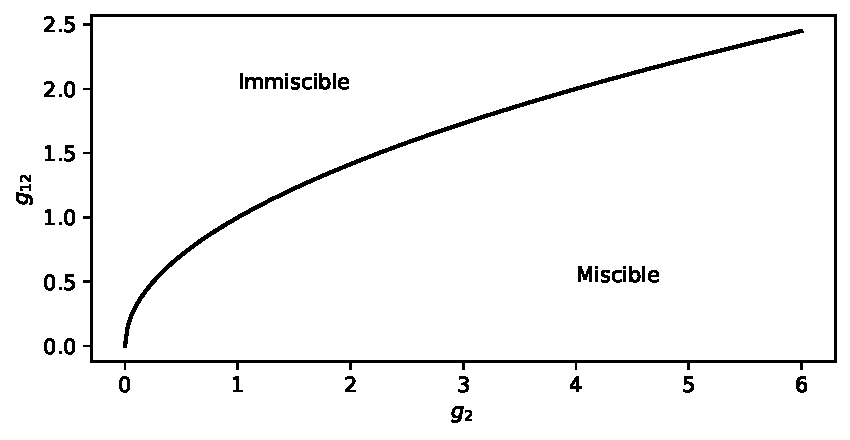
\includegraphics{gfx/ch-theory/miscible_vs_immiscible.pdf}
    \caption[Two-component miscible vs immiscible boundary]
    {\label{fig: miscible-vs-immiscible}Boundary between the miscible
        and immiscible regimes for a two-component condensate with \(g_1=1\).}
\end{figure}


\section{Spinor Bose-Einstein condensates}
Spinor systems comprise particles with total spin \(f\).
This implies there are \(2f + 1\) possible spin states along a given spin
quantisation axis.
Such a state is denoted \(\ket{f, m} \), where
\(m \in \{-f, -f+1, \ldots, 0, \ldots, f - 1, f\} \) denotes the magnetic
sublevel for total spin \( f\).

A general spin-\(f\) state is described by the (\(2f+1\))-component wave
function \(\psi \), defined as \(\ket{\psi} = \sum_m\psi_m\ket{f, m}\).
In the spin-1 case, we have \(\psi = {(\psi_1, \psi_0, \psi_{-1})}^T\), and for
the spin-2 case \(\psi = {(\psi_2, \psi_1, \psi_0, \psi_{-1}, \psi_{-2})}^T\).

Two identical spin-\(f\) bosons (atoms with integer spin) can collide to form a
total spin of \(\EuScript{F} = 0, 2, \ldots, 2f\) depending on the orientation
of the particles, with \(\EuScript{M} \equiv m+m' \in
\{-\EuScript{F}, \ldots, \EuScript{F}\} \).
In the s-wave scattering limit, where the orbital angular momentum is zero,
the total spin of two interacting particles must be even.
Due to the rotational symmetry, the scattering lengths depend only on the total
spin \(\EuScript{F}\), implying there are \(f + 1\) different scattering lengths
\(a_0, a_2, \ldots, a_{2f}\).

In a spinor BEC, the effective contact interaction is generalised to include
contributions from all spin channels as
\begin{equation}\label{eq: spin-f-interaction-potential}
    V_\mathrm{int} = \delta(\vb{r_1} - \vb{r_2})
    \sum_{\EuScript{F}=0}^{2f}g_\EuScript{F}\vb{P}_\EuScript{F},
\end{equation}
where \(g_\EuScript{F}=4\pi\hbar^2a_\EuScript{F}/M\) and
\(\vb{P}_\EuScript{F}\) is the projection operator which projects a pair
of atoms into a total spin \(\EuScript{F}\) state, defined as
\begin{equation}
    \vb{P}_\EuScript{F} = \sum_{m=-\EuScript{F}}^{\EuScript{F}}
    \ket{\EuScript{F}, \EuScript{M}}\bra{\EuScript{F}, \EuScript{M}}.
\end{equation}
For a system of identical bosons, the sum over all projection operators gives
\begin{equation}\label{eq: completeness-relation}
    \sum_{\EuScript{F}=0}^{2f}\vb{P}_\EuScript{F} = 1.
\end{equation}


\subsection{Spin-1 interaction Hamiltonian}\label{subsec: spin-1-int-hamil}
To calculate the spin-dependent mean-field interaction potential, it is common
to relate the projection operators to products of the single-particle spin
operators.
For a spin-1 condensate, the composition law of the angular momentum
gives~\cite{Kawaguchi2012, StamperKurn2013}
\begin{equation}\label{eq: composition-law}
    \vb{F}_1 \cdot \vb{F}_2 = \frac{1}{2}\left[{(\vb{F}_1 + \vb{F}_2)}^2
        - \vb{F}_1^2 - \vb{F}_2^2\right] = \frac{1}{2}\EuScript{F}(\EuScript{F} + 1)
    -f(f+1),
\end{equation}
where \(\vb{F}_i\) is the spin operator for atom \(i\).
From here we can construct the relation \(\vb{F}_1 \cdot \vb{F}_2 =
\sum_{\EuScript{F} = 0}^{2f}\lambda_\EuScript{F}\vb{P}_\EuScript{F}\), where
\(\lambda_\EuScript{F} = \frac{1}{2}\EuScript{F}(\EuScript{F} + 1)
-f(f+1)\).
In an \(f=1\) spinor condensate, only \(\EuScript{F} = 0\) or \(2\) channels
are allowed.
Therefore, we have
\begin{equation}\label{eq: spin-1-spin-relation}
    \vb{F}_1 \cdot \vb{F}_2 = \sum_{\EuScript{F} = 0}^{2f}
    \lambda_\EuScript{F}\vb{P}_\EuScript{F} = \vb{P}_2 - 2\vb{P}_0,
\end{equation}
and
\begin{equation}\label{eq: spin-1-completeness-relation}
    \sum_{\EuScript{F} = 0}^{2f} = 1 = \vb{P}_0 + \vb{P}_2.
\end{equation}
Using both Eq.~\eqref{eq: spin-1-spin-relation} and
Eq.~\eqref{eq: spin-1-completeness-relation}, one can re-write
Eq.~\eqref{eq: spin-f-interaction-potential} as
\begin{equation}
    V_\mathrm{int} = \delta(\vb{r}_1 - \vb{r}_2)
    (c_0 + c_1 \vb{F}_1 \cdot \vb{F}_2),
\end{equation}
where \(c_0 = (g_0+2g_2)/3\) and \(c_1=(g_2-g_0) / 3\).
Finally, the spin-1 interacting Hamiltonian is then given as
\begin{equation}\label{eq: spin-1-interacting-Hamiltonian}
    H_\mathrm{int} = \frac{1}{2}\int d\vb{r} (c_0n^2 + c_1|\vb{F}|^2).
\end{equation}

Here \(c_0\) is interpreted as the spin-independent interaction strength.
It becomes apparent from Eq.~\ref{eq: spin-1-interacting-Hamiltonian} that
\(c_0 > 0\) (repulsive interactions) is required for stability.
In the \(c_0 < 0\) limit (i.e., attractive interactions), the condensate would
favour becoming infinitely dense, and in the process would destroy itself.
Therefore, throughout this thesis we always consider \(c_0 > 0\).

The \(c_1\) term describes is the spin-dependent interaction strength.
Since \(c_0\) is constrained to be positive, \(c_1\) can take positive or
negative values.
When \(c_1 > 0\), the system energetically favours minimising the condensate
spin \(\vb{F}\), which are typically referred to as antiferromagnetic or polar
interactions.
Conversely, for \(c_1 < 0\) the system favours maximising the spin vector,
which are referred to as ferromagnetic interactions.

Finally, we note that since \(c_1\) is the difference of two s-wave scattering
lengths which are comparable in magnitude experimentally, the spin-dependent
interaction strength is usually much smaller than the spin-independent strength.

\subsection{Spin-2 interaction Hamiltonian}
For an \(f=2\) spinor condensate, we now have \(\EuScript{F}=0,2,4\) spin
channels.
For a spin-2 condensate, Eq.~\eqref{eq: composition-law} now gives
\begin{equation}
    \vb{F}_1 \cdot \vb{F}_2 = \sum_{\EuScript{F} = 0}^{2f}
    \lambda_\EuScript{F}\vb{P}_\EuScript{F} = -6\vb{P}_0-3\vb{P}_2+4\vb{P}_4.
\end{equation}
Using the above equation and the completeness relation in
Eq.~\eqref{eq: completeness-relation}, one can write \(\vb{P}_2\) and
\(\vb{P}_4\) in terms of \(\vb{P}_0\) and \(\vb{F}_1 \cdot \vb{F}_2\):
\begin{equation}
    \vb{P}_2 = \frac{1}{7}(4 - \vb{F}_1 \cdot \vb{F}_2 - 10\vb{P}_0), \qquad
    \vb{P}_4 = \frac{1}{7}(3 + \vb{F}_1 \cdot \vb{F}_2 + 3\vb{P}_0).
\end{equation}
From Eq.~\eqref{eq: spin-f-interaction-potential}, the spin-2 interaction
potential takes the form
\begin{equation}
    V_\mathrm{int}\delta(\vb{r}_1-\vb{r}_2)(c_0+c_1\vb{F}_1 \cdot \vb{F}_2
    +c_2\vb{P}_0),
\end{equation}
where \(c_0=(4g_2+3g_4)/7\), \(c_1=(g_4-g_2)/7\), and
\(c_2=(7g_0-10g_2+3g_4)/7\).
Both \(c_0\) and \(c_1\) are the spin-independent and -dependent interaction
strengths, respectively, analogous to the spin-1 system.
Due to the extra degree of freedom in the spin-2 system, a new interaction term,
\(c_2\), describing the spin-singlet interaction arises.

The spin-2 interaction Hamiltonian is given as
\begin{equation}\label{eq: spin-2-interacting-Hamiltonian}
    H_\mathrm{int} = \frac{1}{2}\int d\vb{r}\left(c_0n^2+c_1|\vb{F}|^2
    +c_2|A_{20}|^2\right),
\end{equation}
where \(|A_{20}|^2\) is the spin-singlet duo amplitude, defined in terms of
the condensate wave function as
\begin{equation}
    A_{20} = \frac{1}{\sqrt{5}}\left(\psi_0^2-2\psi_1\psi_{-1}
    +2\psi_2\psi_{-2}\right).
\end{equation}
For \(c_2 > 0\), it becomes energetically favourable to minimise the
spin-singlet amplitude, i.e., \(|A_{20}|^2 = 0\).
Conversely, for interactions where \(c_2 < 0\), the energy is minimised by
maximising the amplitude \(|A_{20}|^2=n/5\).

\subsection{Single-particle Hamiltonian}
When a magnetic field is applied to a spinor system, the field causes energy
shifts in the spin components.
When this field is aligned along the spin quantisation axis, linear, \(p\), and
quadratic, \(q\), Zeeman shifts arise.
In such a case, the single-particle (non-interacting) Hamiltonian is given
by~\cite{Kawaguchi2012}
\begin{equation}\label{eq: single-particle-Hamiltonian}
    H_0 = \int d\vb{r}\sum_{m,m'=-f}^{f} \psi_m^\dagger \left[
        -\frac{\hbar^2}{2M}\nabla^2 + V(\vb{r}) - pm + qm^2\right]\psi_{m'},
\end{equation}
where \(V(\vb{r})\) is a trapping potential.
Throughout most of this thesis we assume that the magnetic field applied is
uniform, such that the Zeeman shifts are constant.
In Chapter~\ref{chap: spin-1}, however, we introduce a time-dependent field
such that the quadratic Zeeman shift has a time-dependence.
Despite the time-dependence, the quadratic Zeeman shift is still spatially
uniform.

It becomes apparent from Eq.~\eqref{eq: single-particle-Hamiltonian} that the
quadratic shift uniformly alters the energetic separation between the
\(\psi_{\pm 1}\) and \(\psi_0\) components.
Conversely, the linear shift maintains the separation.

\section{Spinor Gross-Pitaevskii equations}
\subsection{Spin-1}\label{subsec: spin-1-gpes}
Combing the results of the previous sections, the energy functional of a spin-1
BEC is given as~\cite{Kawaguchi2012}
\begin{equation}\label{eq: spin-1-energy-functional}
    E = \int \left[\sum_{m=-1}^1\psi_m^*\left(-\frac{\hbar^2\nabla^2}{2M}
        + V(\vb{r}) - pm + qm^2\right)\psi_m + \frac{c_0}{2}n^2
        + \frac{c_1}{2}|\vb{F}|^2\right] d^3\vb{r},
\end{equation}
where \(n(\vb{r}) = \sum_{m=-1}^{1}|\psi_m(\vb{r})|^2\) is the total particle
density of the system.
Here, \(\vb{F}=(F_x, F_y, F_z)\) is the spin density vector, defined as
\begin{equation}\label{eq: spinor-spin-vector}
    F_\nu(\vb{r}) = \sum_{m,m'=-1}^{1}\psi_m^*(\vb{r}){(\vb{f}_\nu)}_{mm'}
    \psi_{m'}(\vb{r}), \qquad (\nu=x, y, z).
\end{equation}
The spin-1 Pauli matrices \(\vb{f}_\mu \) are given in the irreducible
representation as
\begin{equation}\label{eq: spin-1-Pauli-matrices}
    \vb{f}_x = \frac{1}{\sqrt{2}}\mqty(0 & 1 & 0 \\ 1 & 0 & 1 \\ 0 & 1 & 0),
    \qquad
    \vb{f}_y = \frac{i}{\sqrt{2}}\mqty(0 & -1 & 0 \\ 1 & 0 & -1 \\ 0 & 1 & 0),
    \qquad
    \vb{f}_z = \mqty(1 & 0 & 0 \\ 0 & 0 & 0 \\ 0 & 0 & -1).
\end{equation}
Substituting Eq.~\eqref{eq: spin-1-Pauli-matrices} into
Eq.~\eqref{eq: spinor-spin-vector} gives the exact expressions of the spin-1
spin vectors:
\begin{align}\label{eq: spin-1-spin-vectors}
    F_x & = \frac{1}{\sqrt{2}} \left(\psi_1^*\psi_0 + \psi_0^*(\psi_1+\psi_{-1})
    + \psi_{-1}^*\psi_0\right)                                                   \\
    F_y & = \frac{i}{\sqrt{2}}\left(-\psi_1^*\psi_0 + \psi_0^*(\psi_1-\psi_{-1})
    +\psi_{-1}^*\psi_0\right)                                                    \\
    F_z & = |\psi_1|^2-|\psi_{-1}|^2.
\end{align}

The spin-1 Gross-Pitaevskii equations are derived, though lengthy, from the
variational derivative of the energy functional in
Eq.~\eqref{eq: spin-1-energy-functional} as \(i\hbar\delta E/\delta \psi_m^*\).
This results in
\begin{equation}\label{eq: spin-1-GPEs}
    i\hbar \pdv{\psi_m}{t} = \left[-\frac{\hbar^2\nabla^2}{2M} + V(\vb{r})
        - pm + qm^2 + c_0n\right]\psi_m
    + c_1\sum_{m'=-1}^{1}\vb{F}\cdot \vb{f}_{mm'}\psi_{m'},
\end{equation}
which describe the mean-field evolution of spin-1 Bose-Einstein condensates.

Time-independent equations are found through the substitution
\(\psi_m = \psi_m(\vb{r})e^{-i\mu t/\hbar}\), where \(\mu \) is the chemical
potential.
Substituting into Eq.~\eqref{eq: spin-1-GPEs} and writing the equation for
each component explicitly gives
\begin{align}\label{eq: spin-1-GPEs-dimensional-psi1}
    \left[-\frac{\hbar^2\nabla^2}{2M} + V(\vb{r}) - p + q + c_0n + c_1F_z
    - \mu\right]\psi_1 + \frac{c_1}{\sqrt{2}}F_-\psi_0    & = 0  \\
    \frac{c_1}{\sqrt{2}}F_+\psi_1 + \left[-\frac{\hbar^2\nabla^2}{2M}
        + V(\vb{r}) + c_0n - \mu\right]\psi_0 + \frac{c_1}{\sqrt{2}}F_-\psi_{-1}
                                                          & = 0  \\
    \left[-\frac{\hbar^2\nabla^2}{2M} + V(\vb{r}) + p + q + c_0n - c_1F_z
    - \mu\right]\psi_{-1} + \frac{c_1}{\sqrt{2}}F_+\psi_0 & = 0,
    \label{eq: spin-1-GPEs-dimensional-psim1}
\end{align}
where \(F_{\pm} = F_x \pm iF_y\).
These equations can be solved to reveal more on the ground states and stationary
solutions of spinor BECs, which forms the basis of
Chapter~\ref{chap: ground-states}.

\subsection{Spin-2}
The spin-2 energy functional is written as~\cite{Kawaguchi2012}
\begin{equation}\label{eq: spin-2-energy-functional}
    E = \int \left[\sum_{m=-2}^{2}\psi_m^* \left(-\frac{\hbar^2\nabla^2}{2M}
    + V(\vb{r}) -pm + qm^2\right)\psi_m + \frac{c_0}{2}n^2
    + \frac{c_1}{2}|\vb{F}|^2 + \frac{c_2}{2}|A_{20}|^2\right] d^3\vb{r}.
\end{equation}
The spin-2 Pauli matrices are given in irreducible representation as
\begin{equation*}
    \vb{f}_x = \mqty(0 & 1  & 0 & 0 & 0 \\
    1 & 0 & \sqrt{\frac{3}{2}} & 0 & 0 \\
    0 & \sqrt{\frac{3}{2}} & 0 & \sqrt{\frac{3}{2}} & 0 \\
    0 & 0 & \sqrt{\frac{3}{2}} & 0 & 1 \\
    0 & 0 & 0 & 1 & 0), \qquad
    \vb{f}_y = \mqty(0 & -i  & 0 & 0 & 0 \\
    i & 0 & -i\sqrt{\frac{3}{2}} & 0 & 0 \\
    0 & i\sqrt{\frac{3}{2}} & 0 & -i\sqrt{\frac{3}{2}} & 0 \\
    0 & 0 & i\sqrt{\frac{3}{2}} & 0 & -i \\
    0 & 0 & 0 & i & 0),
\end{equation*}
\begin{equation}
    \vb{f}_z = \mqty(2 & 0 & 0 & 0 & 0 \\
    0 & 1 & 0 & 0 & 0 \\
    0 & 0 & 0 & 0 & 0 \\
    0 & 0 & 0 & -1 & 0 \\
    0 & 0 & 0 & 0 & -2).
\end{equation}

Similar to the spin-1 case, the GPEs are obtained through the variational
derivative of Eq.~\eqref{eq: spin-2-energy-functional}, resulting in
five coupled equations that model the mean-field dynamics of spin-2
Bose-Einstein condensates.
\begin{align}
    i\hbar\pdv{\psi_{\pm 2}}{t} & = \left[-\frac{\hbar^2\nabla^2}{2M}
        + V(\vb{r}) \mp 2p + 4q + c_0n \pm 2c_1F_z - \mu\right]\psi_{\pm 2}
    + c_1F_{\mp}\psi_{\pm 1} + \frac{c_2}{\sqrt{2}}A_{20}\psi_{\mp 2}^*
    \label{eq: spin-2-GPEs-pm2}                                            \\
    i\hbar\pdv{\psi_{\pm 1}}{t} & = \left[-\frac{\hbar^2\nabla^2}{2M}
        + V(\vb{r}) \mp p + q + c_0n \pm c_1F_z - \mu\right]\psi_{\pm 1}
    + c_1\left(\frac{\sqrt{6}}{2}F_{\mp}\psi_0 + F_{\pm}\psi_{\pm 2}\right)
    - \frac{c_2}{\sqrt{2}}A_{20}\psi_{\mp 1}^* \label{eq: spin-2-GPEs-pm1} \\
    i\hbar\pdv{\psi_0}{t}       & = \left[-\frac{\hbar^2\nabla^2}{2M}
        + V(\vb{r}) + c_0n - \mu\right]\psi_0
    + \frac{\sqrt{6}}{2}c_1\left(F_+\psi_1 + F_-\psi_{-1}\right)
    + \frac{c_2}{\sqrt{2}}A_{20}\psi_{\mp 2}^*, \label{eq: spin-2-GPEs-0}
\end{align}
where the spin vectors are given as
\begin{align}\label{eq: spin-2-spin-vectors}
    F_+ = F_-^* & = 2(\psi_2^*\psi_1 + \psi_{-1}^*\psi_{-2})
    + \sqrt{6}(\psi_1^*\psi_0 + \psi_0^*\psi_{-1}),                             \\
    F_z         & = 2(|\psi_2|^2 - |\psi_{-2}|^2) + |\psi_1|^2 - |\psi_{-1}|^2.
\end{align}

Following the same procedure as in the spin-1 case, the time-independent GPEs
can be found through the substitution
\(\psi_m(\vb{r}, t) = \psi_m(\vb{r})e^{-\mu t/\hbar}\).
\textcolor{red}{Worth listing time-independent GPEs for spin-2 case?}

\subsection{Conserved quantities}
In spinor BECs, there are three conserved quantities.
Firstly, the total energy of the system
    [Eq.~\eqref{eq: spin-1-energy-functional} and
        Eq.~\eqref{eq: spin-2-energy-functional}] is conserved.
In addition, the total atom number of the condensate
\begin{equation}
    N = \int \sum_m |\psi_m|^2 d^3\vb{r}
\end{equation}
is also conserved.
Different from the scalar case, however, is the additional conservation of the
\(z\)-component of the magnetisation
\begin{equation}
    M_z = \int F_z d^3\vb{r},
\end{equation}
where \(F_z\) is given in Eq.~\eqref{eq: spin-1-spin-vectors} or
Eq.~\eqref{eq: spin-2-spin-vectors} for the spin-1 and spin-2 cases,
respectively.
\textcolor{red}{Appendix on derivations?}

\section{Reduction to lower dimensions}
One can reduce the full 3D coupled GPEs to lower dimensions by considering
sufficiently tight confinement of the condensate in one or more directions.
Here, we reduce both the spin-1 and spin-2 GPEs to their 2D and 1D counterparts.

\subsection{Spin-1}
To begin, we start with the full 3D dimensional equations given in
Eqs.~\eqref{eq: spin-1-GPEs-dimensional-psi1} ---
~\eqref{eq: spin-1-GPEs-dimensional-psim1}, written in matrix form as
\begin{align}\label{eq: spin-1-GPEs-matrix}
    i\hbar \pdv{\Psi}{t} = \left[-\frac{\hbar^2\nabla^2}{2M} + V(\vb{r}) + c_0n
    + c_1n \langle\hat{\vb{F}}\rangle \cdot \hat{\vb{F}} - p\hat{F}_z
    + q\hat{F}_z^2\right]\Psi,
\end{align}
where \(\Psi=(\psi_1, \psi_0, \psi_{-1})\) is the three-component wave function.
\textcolor{red}{Has \(\hat{\vb{F}}\) been defined before?}
To reduce the dimensionality, we assume the condensate has been tightly confined
in the \(z\) direction by means of a harmonic oscillator which has trapping
frequencies (\(\omega_x, \omega_y, \omega_z\)) in the (\(x, y, z\)) directions,
respectively.
A tight confinement in the \(z\) direction is achieving by having
\(\omega_z \gg \omega_x, \omega_y\).
In addition, we assume the trapping frequencies are sufficiently such that only
the ground state of the condensate is occupied.
With these assumptions, we can separate the wave function of the condensate into
its 2D counterpart:
\begin{align}\label{eq: Psi-2D}
    \Psi(x, y, z, t) = \tilde{\Psi}(x, y, t)\Phi(z)
    = \sqrt{\tilde{n}(x, y, t)}\zeta(x, y, t)\Phi(z),
\end{align}
where \(\Phi(z)\) is normalised as \(\int_{-\infty}^{\infty}|\Phi(z)|^2 \, \dd z
= 1\), and we apply the single-mode approximation (SMA) such that
\(\zeta(x, y, t)\) has no \(z\)-dependence.

Substituting Eq.~\eqref{eq: Psi-2D} into Eq.~\eqref{eq: spin-1-GPEs-matrix} we
obtain
\begin{equation}
\begin{split}
    i\hbar\pdv{\tilde{\Psi}}{t}\Phi = \left[
        -\frac{\hbar^2}{2M}\Phi\nabla_\perp^2
        - \frac{\hbar^2}{2M}\pdv[2]{\Phi}{z} + [V_\perp(x, y) + V_z(z)]\Phi
        +c_0\tilde{\Psi}^\dagger\tilde{\Psi}|\Phi|^2\Phi\right. \\
        \left.+c_1\tilde{\Psi}^\dagger\tilde{\Psi}|\Phi|^2\Phi
        \langle\hat{\vb{F}}\rangle \cdot \hat{\vb{F}}
        -p\Phi\hat{F}_z + q\Phi\hat{F}_z^2 \vphantom{\int_1^2}\right]\Psi.
\end{split}
\end{equation}
To reduce the equation further, we multiply from the left by \(\Phi^*\) and
integrate over the \(z\) direction, which gives:
\begin{equation}\label{eq: spin-1-GPEs-tildes}
\begin{split}
    \left[
        -\frac{\hbar^2}{2M}\Phi\nabla_\perp^2
        - \frac{\hbar^2}{2M}\int_{-\infty}^{\infty}\Phi^*\dv[2]{\Phi}{z} \dd z
        + V_\perp(x, y) + \int_{-\infty}^{\infty} V_z(z)|\Phi|^2 \dd z\right. \\
        \left.+c_0\tilde{n}\int_{-\infty}^{\infty}|\Phi|^4 \dd z
        +c_1\tilde{n}\langle\hat{\vb{F}}\rangle \cdot \hat{\vb{F}}
        \int_{-\infty}^{\infty}|\Phi|^4 \dd z
        -p\hat{F}_z + q\Phi\hat{F}_z^2 \right]\Psi.
\end{split}
\end{equation}
In the above equation, the constant \(C =
-\frac{\hbar^2}{2M}\int_{-\infty}^{\infty}\Phi^*\dv[2]{\Phi}{z} \dd z
+ \int_{-\infty}^{\infty} V_z(z)|\Phi|^2 \dd z\) can be removed from the
equation via the appropriate transformation \(\tilde{\Psi} \rightarrow
\tilde{\Psi}e^{-Ct/N}\), where \(N\) is the total atom number.
Now, we take \(\Phi(z)\) to be the harmonic oscillator ground state, which has
the form
\begin{align}
    \Phi(z) =
    {\left(\frac{\beta}{\pi}\right)}^{\frac{1}{4}}e^{-\frac{\beta}{2}z^2},
\end{align}
where \(\beta = M\omega_z/\hbar \).
This then leads to the integral
\begin{align}
    \int_{-\infty}^{\infty}|\Phi(z)|^4 \dd z = \sqrt{\frac{\beta}{2\pi}}.
\end{align}
We can then appropriately rescale the interaction strengths into their 2D
counterparts:
\begin{align}
    c_0^\text{2D} = c_0\sqrt{\frac{\beta}{2\pi}}, \qquad
    c_1^\text{2D} = c_1\sqrt{\frac{\beta}{2\pi}}.
\end{align}
Finally, substituting back into Eq.~\eqref{eq: spin-1-GPEs-tildes} yields the
2D GPEs for a spin-1 system:
\begin{align}
    i\hbar\pdv{\Psi}{t} = \left[-\frac{\hbar^2}{2M}\nabla_\perp^2 + V_\perp
    + c_0^\text{2D}n + c_1^\text{2D}n\langle\hat{\vb{F}}\rangle \cdot \hat{\vb{F}}
    -p\hat{F}_z + q\hat{F}_z^2\right]\Psi,
\end{align}
where we have dropped the tildes for notational convenience.

A similar process can be used to reduce the full 3D equations into their 1D
counterparts.
We now assume that the condensate is tightly confined in two directions, which
we will take to be the \(x, y\) directions (\(\omega_x, \omega_y \gg
\omega_z\)).
This time, we separate the wave function according to
\begin{align}
    \Psi(x, y, z, t) = \tilde{\Psi}(z, t)\Phi(x, y) = \sqrt{\tilde{n}(z, t)}
    \zeta(z, t)\Phi(x, y),
\end{align}
once again assuming \(\Phi(x, y)\) to be normalised as \(\int_{-\infty}^{\infty}
\int_{-\infty}^{\infty} |\Phi(x, y)|^2 \dd x \dd y = 1\) and using the SMA such
that \(\zeta(z, t)\) only has a \(z\) dependence.
We substitute the above expression in the GPEs
(Eq.~\eqref{eq: spin-1-GPEs-matrix}) and find
\begin{equation}
\begin{split}
    i\hbar\pdv{\tilde{\Psi}}{t}\Phi = \left[
        -\frac{\hbar^2}{2M}\Phi\pdv[2]{}{z}
        - \frac{\hbar^2}{2M}\nabla_\perp^2\Phi + [V_\perp(x, y) + V_z(z)]\Phi
        +c_0\tilde{\Psi}^\dagger\tilde{\Psi}|\Phi|^2\Phi\right. \\
        \left.+c_1\tilde{\Psi}^\dagger\tilde{\Psi}|\Phi|^2\Phi
        \langle\hat{\vb{F}}\rangle \cdot \hat{\vb{F}}
        -p\Phi\hat{F}_z + q\Phi\hat{F}_z^2 \vphantom{\int_1^2}\right]\Psi.
\end{split}
\end{equation}
Following the procedure before, we multiply from the left by \(\Phi^*\)
and integrate over \(x\) and \(y\) which yields
\begin{equation}
\begin{split}
    \left[
        -\frac{\hbar^2}{2M}\Phi\pdv[2]{}{z}
        - \frac{\hbar^2}{2M}\int_{-\infty}^{\infty}\int_{-\infty}^{\infty}
        \Phi^*\dv[2]{\Phi}{z} \dd x \dd y
        + V_\perp(x, y) + \int_{-\infty}^{\infty}\int_{-\infty}^{\infty}
        V_z(z)|\Phi|^2 \dd x \dd y\right. \\
        \left.+c_0\tilde{n}\int_{-\infty}^{\infty}\int_{-\infty}^{\infty}
        |\Phi|^4 \dd x \dd y
        +c_1\tilde{n}\langle\hat{\vb{F}}\rangle \cdot \hat{\vb{F}}
        \int_{-\infty}^{\infty}\int_{-\infty}^{\infty}|\Phi|^4 \dd x \dd y
        -p\hat{F}_z + q\Phi\hat{F}_z^2 \right]\Psi.
\end{split}
\end{equation}
Now, the constant term \(C = -\hbar^2/2M\int_{\infty}^{\infty}
\int_{\infty}^{\infty}|\nabla_\perp^2\Phi|^2\dd x \dd z
+\int_{\infty}^{\infty}\int_{\infty}^{\infty}V_\perp|\Phi|^2\dd x \dd y\) can
again be dropped from the equation via the appropriate substitution
\(\tilde{\Psi} = \tilde{\Psi}e^{-iCt/N}\).
We then take \(\tilde{\Psi}\) to be the lowest harmonic oscillator ground state,
which in 2D becomes
\begin{align}
    \Phi(x, y) = {\left(\frac{\beta}{\pi}\right)}^{1/2}
    e^{-\frac{\beta}{2}(x^2+y^2)},
\end{align}
where \(\beta=m\omega_\perp / \hbar \), which leads to the relation
\begin{align}
    \int_{\infty}^{\infty}\int_{\infty}^{\infty} |\Phi(x, y)|^4 \dd x \dd y
    = \frac{\beta}{2\pi}.
\end{align}
This then leads to the 1D rescaled interaction strengths
\begin{align}
    c_0^\text{1D} = c_0\frac{\beta}{2\pi}, \qquad
    c_1^\text{1D}=c_1\frac{\beta}{2\pi}.
\end{align}
Finally, we arrive at the 1D GPE given in matrix form:
\begin{align}
    i\hbar\pdv{\Psi}{t} = \left[-\frac{\hbar^2}{2M}
    \pdv[2]{}{z}+V_z(z) + c_0^\text{1D}n
    + c_1^\text{1D}\langle\hat{\vb{F}}\rangle \cdot \hat{\vb{F}} - p\hat{F}_z
    + q\hat{F}_z^2\right]\Psi,
\end{align}
again dropping the tildes for notational convenience.

\section{Dimensionless spinor Gross-Pitaevskii equations}
\label{sec: dimensionless-equations}
Systems that can undergo Bose-Einstein condensation, and hence become a
superfluid, can form at a variety of length scales, ranging from Bose-Einstein
condensates at the micron scale all the way to the cores of neutron stars,
which are theorised to be superfluid on the kilometre
scale~\cite{Warszawski2011}.
In addition, atomic Bose-Einstein condensates in experiment take on a wide range
of variable parameters and geometries.
Such geometries include box-like potentials~\cite{Gaunt2013}, toroidal ring
geometries~\cite{Ryu2007, Ramanathan2011}, both quasi-2D~\cite{Neely2010}
and quasi-1D systems~\cite{Burger1999}, and even arbitrary
potentials~\cite{Henderson2009}.

Due to these reasons, rescaling the quantities used in the corresponding GPEs
allows one to reformulate any calculation into a desired scale and parameter
regime.
In practice, this is done by casting the GPEs into a dimensionless form, where
each dimensional parameter in the equation is rescaled using an appropriate
quantity such that it becomes dimensionless.
An advantage of using a dimensionless form is that the parameters used within
numerical computation become normalised on the scale of unity, which,
when compared to values in the dimensional equation such as \(\hbar =
1.054\times 10^{-34}\), can reduce numerical errors that arise due to the
floating point representation used by computers.

The process of making the GPEs dimensionless can be done in different ways,
where the scaling parameters chosen typically depend on whether the system is
trapped or not.
Here, we derive the dimensionless 3D GPEs for both a homogeneous spin-1 BEC and
a trapped spin-2 BEC, which will aid the analysis in subsequent chapters.

\subsection{Homogeneous spin-1 BEC}
Consider a homogeneous system in the absence of a trapping potential
\(V(\vb{r}) = 0\).
In a spin-1 system, there are two choices of length scales one
can choose as their unit of length: the density healing length
\(\xi_d=\hbar /\sqrt{2Mc_0n_0}\), or the spin healing length
\(\xi_s = \hbar /\sqrt{2M|c_1|n_0}\), where \(n_0\) is the background density
of the uniform system.
Both choices are valid, but for this thesis we shall choose the spin healing
length, \(\xi_s\).
Then, an appropriate unit of energy is the spin energy: \(E_s = 2|c_1|n_0\),
which leads to the spin time \(\tau_s = \hbar / E_s\).
Now we have found appropriate units for length, time, and energy, we can
rescale each quantity as
\begin{align}
    \vb{r} \rightarrow \xi_s \tilde{\vb{r}}, \qquad
    t \rightarrow \tau_s\tilde{t}, \qquad
    \Psi \rightarrow \sqrt{n_0}\tilde{\Psi},
\end{align}
where a tilde denotes the dimensionless quantity.
Substituting these into Eq.~\eqref{eq: spin-1-GPEs-matrix} leads to the
dimensionless spin-1 GPEs:
\begin{align}
    i \pdv{\tilde{\psi}_{1}}{\tilde{t}} &= \left[-\frac{1}{2}\tilde{\nabla}^2
    + \tilde{c}_0\tilde{n} + \tilde{c}_1\tilde{n}\tilde{F}_z - \tilde{p}
    + \tilde{q}\right]\tilde{\psi}_{1}
    + \frac{\tilde{c}_1}{\sqrt{2}}\tilde{F}_-\tilde{\psi}_0, \\
    i \pdv{\tilde{\psi}_0}{\tilde{t}} &= \left[-\frac{1}{2}\tilde{\nabla}^2
    + \tilde{c}_0\tilde{n}\right]\tilde{\psi}_0
    + \frac{\tilde{c}_1}{\sqrt{2}}\left(\tilde{F}_+\tilde{\psi}_1
    + \tilde{F}_-\tilde{\psi}_{-1}\right), \\
    i \pdv{\tilde{\psi}_{-1}}{\tilde{t}} &= \left[-\frac{1}{2}\tilde{\nabla}^2
    + \tilde{c}_0\tilde{n} - \tilde{c}_1\tilde{n}\tilde{F}_z + \tilde{p}
    + \tilde{q}\right]\tilde{\psi}_{-1}
    + \frac{\tilde{c}_1}{\sqrt{2}}\tilde{F}_+\tilde{\psi}_0, \\
\end{align}
where the rescaled interaction strengths and Zeeman shifts are
\begin{align}
    \tilde{c}_0 = \frac{n_0c_0}{E_s} = \left|\frac{c_0}{2c_1}\right|, \quad
    \tilde{c}_1 = \frac{n_0c_1}{E_s} = \frac{1}{2} \cdot \text{sgn}(c_1),\quad
    \tilde{p} = \frac{q}{E_s}, \quad
    \tilde{q} = \frac{q}{E_s}.
\end{align}
By choosing our unit of length and time as \(\xi_s\) and \(\tau_s\),
respectively, the dimensionless spin-dependent interaction strength is fixed
at \(|\tilde{c}_1| = 1/2\).
Therefore, to set the spin-independent interaction strength, \(\tilde{c}_0\),
we need the ratio of the interaction strengths, \(c_0/c_1\), which is set by
the atomic species itself.

\subsection{Trapped spin-2 BEC}
Consider now a spin-2 BEC trapped by a uniform harmonic trap \(V(\vb{r})\).
Now, instead of choosing the healing length as our unit of length, it makes more
sense to instead choose the harmonic oscillator length \(\ell =
\sqrt{\hbar/(M\omega)}\), where \(\omega \) is the trapping frequency.
Then, time is measured in units of \(omega^{-1}\) and energy in
\(\hbar\omega \), which leads to the rescaling of the following units:
\(\vb{r}\rightarrow \ell\tilde{\vb{r}},\ t \rightarrow \omega\tilde{t}\).
To construct the dimensionless wave function, it is conventional to define the
dimensionless wave function as being normalised to unit
\(\int_{-\infty}^\infty |\tilde{\Psi}|^2\dd^3\tilde{\vb{r}} = 1\).
Then, recalling that the dimensional wave function is normalised to the number
of atoms \(\int_{-\infty}^\infty |{\Psi}|^2\dd^3{\vb{r}} = N\), and that
\(\dd^3\vb{r} = \ell^3\dd^3\tilde{\vb{r}}\), it follows that the dimensional
wave function can be rescaled as
\begin{align}
    \Psi \rightarrow \sqrt{\frac{N}{\ell^3}}\tilde{\Psi}.
\end{align}
Substituting these rescaled quantities into Eqs.~\eqref{eq: spin-2-GPEs-pm2}
-~\eqref{eq: spin-2-GPEs-0} yields the dimensionless spin-2 GPEs for a trapped
system
\begin{align}
    i\pdv{\tilde{\psi}_{\pm 2}}{\tilde{t}} &= \left[-\frac{1}{2}\tilde{\nabla}^2
    +V(\tilde{\vb{r}}) \tilde{c}_0\tilde{n} \pm 2\tilde{c}_1\tilde{F}_z
    \mp 2\tilde{p} + 4\tilde{q}\right]\tilde{\psi}_{\pm 2}
    + \tilde{c}_1\tilde{F}_\mp\tilde{\psi}_{\pm 1}
    + \frac{\tilde{c}_2}{\sqrt{2}}\tilde{A}_{20}\tilde{\psi}_{\mp 2}^* \\
    i\pdv{\tilde{\psi}_{\pm 1}}{\tilde{t}} &= \left[-\frac{1}{2}\tilde{\nabla}^2
    +V(\tilde{\vb{r}}) \tilde{c}_0\tilde{n} \pm \tilde{c}_1\tilde{F}_z
    \mp 2\tilde{p} + 4\tilde{q}\right]\tilde{\psi}_{\pm 1}
    +\tilde{c}_1\left(\frac{\sqrt{6}}{2}\tilde{F}_\mp \tilde{\psi}_0
    +\tilde{F}_\pm\tilde{\psi}_{\pm 2}\right)
    - \frac{\tilde{c}_2}{\sqrt{2}}\tilde{A}_{20}\tilde{\psi}_{\mp 1}^* \\
    i\pdv{\tilde{\psi}_0}{\tilde{t}} &= \left[-\frac{1}{2}\tilde{\nabla}^2
    +V(\tilde{\vb{r}})+\tilde{c}_0\tilde{n}\right]\tilde{\psi}_0
    +\frac{\sqrt{6}}{2}\tilde{c}_1\left(\tilde{F}_+\tilde{\psi}_1
    +\tilde{F}_-\tilde{\psi}_{-1}\right)
    + \frac{\tilde{c}_2}{\sqrt{2}}\tilde{A}_{20}\tilde{\psi}_{\pm 2}^*,
\end{align}
where now the rescaled interaction strengths and Zeeman shifts are
\begin{align}\label{eq: spin-2-interaction-strengths-dimensionless}
    \tilde{c}_0 = \frac{Nc_0}{\hbar\omega\ell^3}, \quad
    \tilde{c}_1 = \frac{Nc_1}{\hbar\omega\ell^3}, \quad
    \tilde{c}_2 = \frac{Nc_2}{\hbar\omega\ell^3}, \quad
    \tilde{p} = \frac{p}{\hbar\omega}, \quad
    \tilde{q} = \frac{q}{\hbar\omega}.
\end{align}

\subsection{Mapping to experimental parameters}
Numerical simulations are an extremely useful tool for gaining insight into
what experiments of BEC systems might look like.
Therefore, it is useful to calculate the values of the interaction strengths
for different atomic species so that they can be mapped to our dimensionless
parameters.
In particular, we investigate both the spin-1 and spin-2 atoms of \( ^{23}\)Na
and \( ^{87}\)Rb.
Here, we are taking our unit of length and time to be the harmonic oscillator
length \(\ell \) and inverse trap frequency \(\omega^{-1}\), respectively.

\subsection{Spin-1}
Recall that the dimensional interaction strengths for a spin-1 system are given
as
\begin{align}\label{eq: spin-1-interaction-strengths}
    c_0 = \frac{4\pi\hbar^2}{3M}(a_0+2a_2), \qquad
    c_1 = \frac{4\pi\hbar^2}{3M}(a_2-a_0), \qquad
\end{align}
where \(a_\mathcal{F}\) is the s-wave scattering length for the
spin-\(\mathcal{F}\) channel.
To calculate the dimensional interaction strengths, we list the scattering
lengths obtained by Crubellier~\cite{Crubellier1999} for \( ^{23}\)Na and
Ho~\cite{Ho1998} for \( ^{87}\)Rb in
Table~\ref{table: scaterring-lengths-spin-1}.
\begin{table}[htbp]
    \centering
    \begin{tabular}{ cccc } 
     \toprule
      & \(a_0\) & \(a_2\) \\
      \midrule
      \( ^{23}\)Na & \(50.0\pm 1.6\) & \(55.0\pm 1.7\) \\ 
      \( ^{87}\)Rb & \(110.0\pm 4.0\) & \(107.0\pm 4.0\) \\
      \bottomrule
    \end{tabular}
    \caption{\label{table: scaterring-lengths-spin-1}Table of scattering lengths
    for spin-1 atomic species \( ^{23}\)Na and \( ^{87}\)Rb in units of the Bohr
    radius.}
\end{table}
With these values, we are free to calculate the dimensional interaction
strengths using Eq.~\eqref{eq: spin-1-interaction-strengths}.
To calculate the numerical, dimensionless interaction strengths we assume an
atom number of \(N = 2\times10^5\) and a trapping frequency of
\(\omega = 2\pi \times 130\)Hz.
Both the dimensional (with uncertainties) and dimensionless values for a spin-1
\( ^{23}\)Na system are given in Table~\ref{table: spin-1-interactions-sodium}.
\begin{table}[!htbp]
    \centering
    \begin{tabular}{ccc}
        \toprule
        \( ^{23}\)Na & Dimensional (units of \(\text{kg}\, \text{m}^5
        \text{s}^{-2}\)) & Dimensionless \\
        \midrule
        \(c_0\) & \(1.03 \pm 0.00321 \times 10^{-50}\) & \(3.91\times10^3\) \\
        \(c_1\) & \(3.21 \pm 0.0640 \times 10^{-52}\) & \(122\) \\
        \bottomrule
    \end{tabular}
    \caption{\label{table: spin-1-interactions-sodium}Dimensional (with
    uncertainties) and dimensionless interaction strengths of \( ^{23}\)Na.}
\end{table}
Calculating the ratio of interaction parameters gives \(c_0/c_1=32.0 \),
which predicts the ground state of \( ^{23}\)Na to be polar (see
Sec~\ref{sec: ground-states-spin-1} for details on spin-1 ground states).

For the \( ^{87}\)Rb system, we again assume an atom number of
\(N = 2\times 10^5\) with a trapping frequency of
\(\omega = 2\pi \times 130\)Hz.
The dimensional (with uncertainties) and dimensionless interaction strengths
for a spin-1 \( ^{87}\)Rb are given in
Table~\ref{table: spin-1-interactions-rb87}.
\begin{table}[!htbp]
    \centering
    \begin{tabular}{ccc}
        \toprule
        \( ^{87}\)Rb & Dimensional (units of \(\text{kg}\, \text{m}^5
        \text{s}^{-2}\)) & Dimensionless \\
        \midrule
        \(c_0\) & \(5.43 \pm 0.201 \times 10^{-51}\) & \(2.10\times10^3\) \\
        \(c_1\) & \(-5.03 \pm 10.3 \times 10^{-53}\) & \(-19.1\) \\
        \bottomrule
    \end{tabular}
    \caption{\label{table: spin-1-interactions-rb87}Dimensional (with
    uncertainties) and dimensionless interaction strengths of \( ^{23}\)Na.}
\end{table}
Calculating the ratio of interaction strengths for this system gives
\(c_0/c_1=-110 \), which predicts the ground state of \( ^{87}\)Rb to be
ferromagnetic (see
Sec~\ref{sec: ground-states-spin-1} for details on spin-1 ground states).

\subsection{Spin-2}
Recall that the dimensional interaction strengths for a spin-2 system are given
as
\begin{align}\label{eq: spin-2-interaction-strengths}
    c_0 = \frac{4\pi\hbar^2}{7M}(4a_2+3a_4), \qquad
    c_1 = \frac{4\pi\hbar^2}{7M}(a_4-a_2), \qquad
    c_2 = \frac{4\pi\hbar^2}{7M}(7a_0-10a_2+3a_4),
\end{align}
To determine the values of the interaction strengths, we first list the s-wave
scattering lengths in units of the Bohr radius given by
Ciobanu~\cite{Ciobanu2000} for \( ^{23}\)Na and Klausen~\cite{Klausen2001} for
\( ^{85}\)Rb and \( ^{87}\)Rb in Table~\ref{table: scaterring-lengths-spin-2}.
\begin{table}[htbp]
    \centering
    \begin{tabular}{ cccc } 
     \toprule
      & \(a_0\) & \(a_2\) & \(a_4\) \\
      \midrule
      \( ^{23}\)Na & \(34.9\pm 1.0\) & \(45.8\pm 1.1\) & \(64.5\pm 1.3\) \\ 
      \( ^{85}\)Rb  & \(-740\pm60.0\) & \(-570\pm 50.0\) & \(-390\pm20.0\) \\ 
      \( ^{87}\)Rb & \(86.2\pm 1.0\) & \(90.2\pm 1.0\) & \(97.4\pm 1.0\) \\
      \bottomrule
    \end{tabular}
    \caption{\label{table: scaterring-lengths-spin-2}Table of scattering lengths
    for spin-2 atomic species \( ^{23}\)Na, \( ^{85}\)Rb, and \( ^{87}\)Rb in
    units of the Bohr radius.}
\end{table}
With these scattering lengths we can calculate the dimensional interaction
strengths using Eq.~\eqref{eq: spin-2-interaction-strengths}.
To calculate the corresponding dimensionless interaction strength, we assume
\(N = 2\times10^5\) and \(\omega = 2\pi \times 130\) Hz.
Both the dimensional (with uncertainties) and dimensionless values for a spin-2
\( ^{23}\)Na system are given in
Table~\ref{table: spin-2-interactions-sodium}.
\begin{table}[!htbp]
    \centering
    \begin{tabular}{ccc}
        \toprule
        \( ^{23}\)Na & Dimensional (units of \(\text{kg}\, \text{m}^5
        \text{s}^{-2}\)) & Dimensionless \\
        \midrule
        \(c_0\) & \(1.03 \pm 0.00654 \times 10^{-50}\) & \(3.91\times10^3\) \\
        \(c_1\) & \(5.10 \pm 0.654 \times 10^{-52}\) & \(195\) \\
        \(c_2\) & \(-5.51 \pm 0.927 \times 10^{-52}\) & \(-210\) \\
        \bottomrule
    \end{tabular}
    \caption{\label{table: spin-2-interactions-sodium}Dimensional (with
    uncertainties) and dimensionless interaction strengths of \( ^{23}\)Na.}
\end{table}
The ratios of interaction parameters are
\begin{equation}
    \frac{c_0}{c_1} = 20.1, \qquad \frac{c_0}{c_2} = -18.6,
\end{equation}
which predicts the ground state of \( ^{23}\)Na to be nematic (see
Sec~\ref{sec: ground-state-spin-2} for details).

For \( ^{87}\)Rb we once again assume an atom number of \(N=2\times10^5\) with a
trapping frequency \(\omega = 2\pi \times 130\)Hz.
The dimensional (with uncertainties) and dimensionless parameters for a spin-2
\( ^{87}\)Rb system are listed in
Table~\ref{table: spin-2-interactions-rb87}.
\begin{table}[!htbp]
    \centering
    \begin{tabular}{ccc}
        \toprule
        \( ^{87}\)Rb & Dimensional (units of \(\text{kg}\, \text{m}^5
        \text{s}^{-2} \)) & Dimensionless \\
        \midrule
        \(c_0\) & \(4.71 \pm 0.0144 \times 10^{-51}\) & \(1.32\times10^4\) \\
        \(c_1\) & \(5.19 \pm 1.44 \times 10^{-53}\) & \(146\) \\
        \(c_2\) & \(-4.61 \pm 2.16 \times 10^{-53}\) & \(-129\) \\
        \bottomrule
    \end{tabular}
    \caption{\label{table: spin-2-interactions-rb87}Dimensional (with
    uncertainties) and dimensionless interaction strengths of \( ^{87}\)Rb.}
\end{table}
In this case, the interaction strength ratios are
\begin{align}
    \frac{c_0}{c_1} = 90.7, \qquad \frac{c_0}{c_2} = -102.0,
\end{align}
which again predict the ground state to be nematic (see
Sec~\ref{sec: ground-state-spin-2} for details).
